\chapter{Implementation and Results}
\label{implementation}
This chapter presents an implementation of PIVOT and discusses the results \cite{terenzi}.

\section{Implementation}
\label{implementation_2}
To evaluate PIVOT, we simulated a real-time LoRaWAN network. In detail, our simulator is composed of the \textit{generator}, that produces fake LoRa packets, and \textit{pivot}, that receives and analyzes them.

\begin{figure}
    \centering
    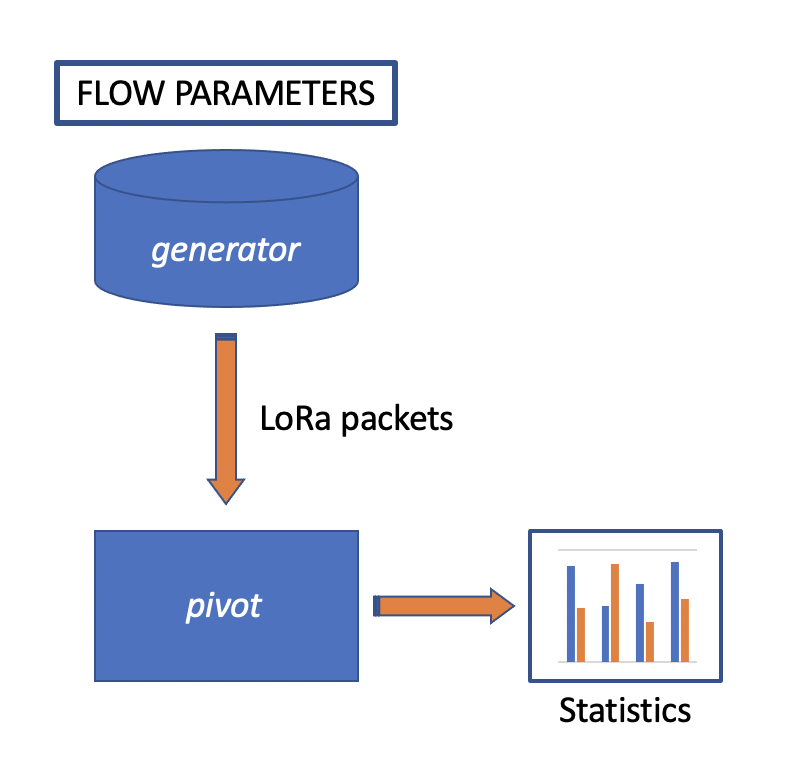
\includegraphics[width=0.5\linewidth]{images/implementation/simulator.png}
    \caption{The architecture of the simulator}
    \label{fig:simulator}
\end{figure}

\subsubsection{\textit{generator}}
In \textit{generator} we can set the number of devices to insert in the network, the periodic pattern they had to follow, and the number of re-joins each of them can make. 

\subsubsection{\textit{pivot}}
As detailed in the previous section, to reduce the detection rate of PIVOT, the operator can change the pattern of vulnerable devices. We reported this scenario in our simulator: when \textit{pivot} alerts about a device, the \textit{generator} modifies its pattern, randomly changing the length of the segments.

\subsection{Code snippets}
In this section, we report and comment the main code snippets of our simulator.
\subsubsection{Packet class}
\begin{mintedbox}[samepage]{python}
class Packet:
	def __init__(self, t, dev, devaddr, rssis, uid, fcnt, mtype, info=""):
		self.rssis = rssis  #can be None, if unavailable
		self.dev_eui = dev
		self.dev_addr = devaddr
		self.t = t
		self.uid = uid
		self.fcnt = fcnt
		self.mtype = mtype
		self.info = info
\end{mintedbox}


\subsubsection{Traffic parameters}
\begin{mintedbox}{python}
N = 300     # number of devices
S = 365*24*3600     # number of seconds to generate packets
Tmin = int(10)      # minimum interarrival time, in seconds
Tmax = int(23*3600)     # maximum interarrival time, in seconds
Emin = 0.01     # minimum absolute error in the interarrival time, in seconds
Emax = 2        # maximum absolute error in the interarrival time, in seconds
P = 10      # maximum length of a pattern
Jmin = 20       # minimum number of messages before a join
Jmax = 300      # maximum number of messages before a join
\end{mintedbox}

\subsubsection{Pattern class}
\begin{mintedbox}[samepage]{python}
class Pattern:
    def __init__(self, timestamp):
        self.timestamp = timestamp
        self.verified = False
        self.segments = []
\end{mintedbox}

\subsubsection{Segment class}
\begin{mintedbox}[samepage]{python}
class Segment:
    def __init__(self, value, index):
        self.n = 1
        self.index = index
        self.mean = value
\end{mintedbox}

\subsubsection{PIVOT class}
\begin{mintedbox}[samepage]{python}
class PIVOT:
    def __init__(self):
        self.confirmed = {}
        self.unconfirmed = {}
        self.quarantine = {}

        self.to_analyze = {}
        self.current_section = 1
\end{mintedbox}

\subsubsection{PIVOT functions}
\begin{mintedbox}{python}
def read_packet(self, p):
    if (p.mtype == "Join Request"):
        self.current_section += 1

    else:
        if self.current_section == 1:
            self.__pre_join(p)
        else:
            self.__post_join(p)  
\end{mintedbox}
\begin{mintedbox}[samepage]{python}
def __pre_join(self, p):
    devaddr = p.dev_addr

    if devaddr in self.confirmed:
        self.confirmed[devaddr].update(p.t)
    else:
        self.confirmed[devaddr] = Pattern(p.t)
\end{mintedbox}
\begin{mintedbox}{python}
def __main_procedure(self, p):
    
    # gets the Dev Address
    devaddr = p.dev_addr  
    
    # checks if the pattern already exists
    if devaddr in self.confirmed:
        self.confirmed[devaddr].update(p.t)
        self.__clean(devaddr)

    else:
        # check if the DevAddress has already been received
        if devaddr in self.unconfirmed:
            self.unconfirmed[devaddr].update(p.t)
            
            # checks if the DevAddress is in Quarantine
            if devaddr in self.quarantine:
                self.__quarantine(devaddr, p.t)

            else:
                # cheks if the pattern associated with the DevAddress matches with other patterns 
                to_analyze = self.to_analyze[devaddr]
                unconf_pattern = self.unconfirmed[devaddr]


                verified = list(filter(lambda x: self.confirmed[x].verified, to_analyze))

                for v in verified:
                    conf_pattern = self.confirmed[v]        

                    if len(unconf_pattern.segments) == len(conf_pattern.segments):
                        pattern_matching = conf_pattern.contains(unconf_pattern)
                    
                        if pattern_matching:
                            # there is a match, the DevAddress is put in Quarantine        
                            self.quarantine[devaddr] = (v, p.t)      
                        else:
                            self.to_analyze[devaddr].remove(v)

                if len(self.to_analyze[devaddr]) == 0:
                    self.__new_device(devaddr, unconf_pattern)   

        else:
            # initializing a new pattern
            self.unconfirmed[devaddr] = Pattern(p.t)
            self.to_analyze[devaddr] = list(self.confirmed.keys()
\end{mintedbox}

\section{Results}
\label{results}
\subsubsection{Metrics}
PIVOT evaluates the number of vulnerable devices it identifies using the performance metrics of the Precision-Recall curve. In detail, given the following quantities:
\begin{itemize}
	\item True Positive (TP): number of correct re-identifications. 
	\item False Positive (FP): number of false re-identifications.
	\item False Negative (FN): number of missing re-identifications.
\end{itemize}

\begin{figure}
    \centering
    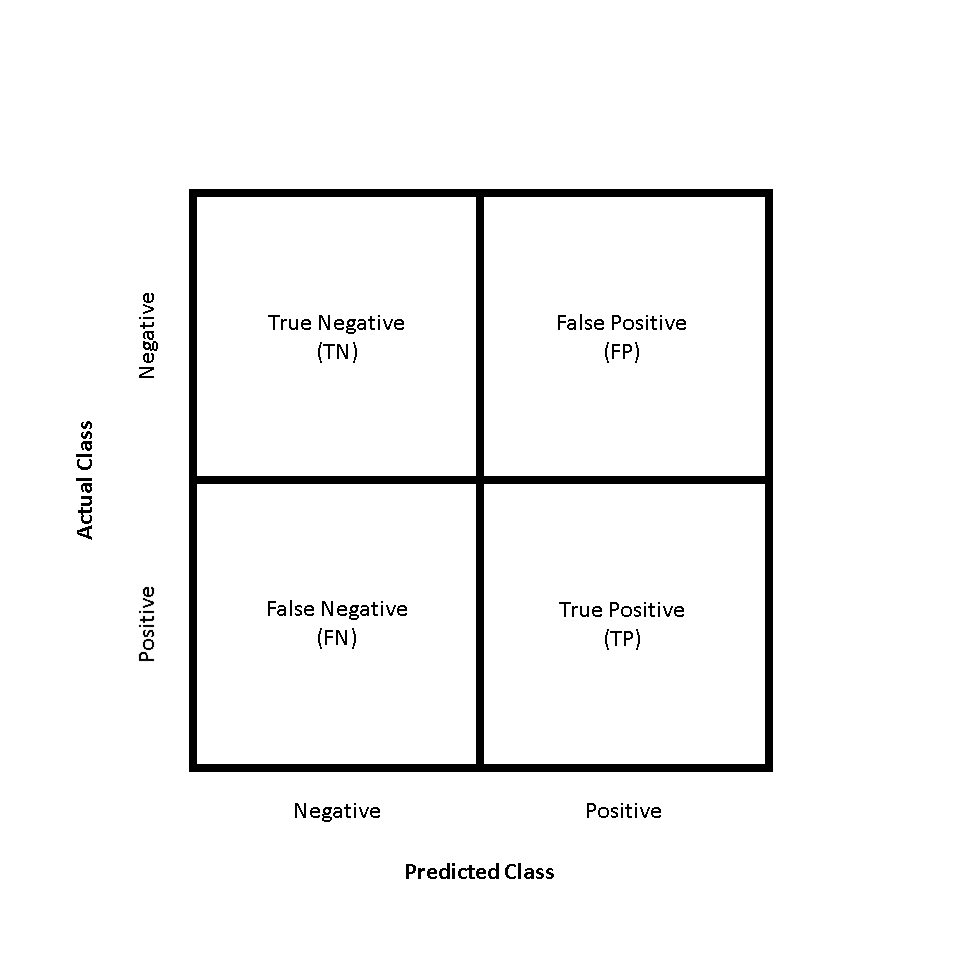
\includegraphics[width=0.7\linewidth]{images/implementation/binary_classification.png}
    \caption{Confusion matrix structure for binary classification problems}
    \label{fig:classification}
\end{figure}


\subsubsection{Precision-Recall curve}
The \textbf{Precision}, also known as Positive Predictive Value, is represented as:
\[\ Precision = PPV = \frac{TP}{TP + FP} \] 
The \textbf{Recall}, also known as \textit{sensitivity}, is represented as:
\[ Recall = sensivity = \frac{TP}{TP + FN} \] 